Unser Projekt zur Analyse von Tweet-Retweet-Beziehungen soll aus drei separaten Programmen bestehen. Dabei sollen die verschiedenen Programme nur über eine zentrale Datenbank miteinander interagieren. Die erste Komponente, der Crawler ist für das Sammeln der Daten von Twitter zuständig, die zweite Komponente, der Kategorisierer ist für eine thematische Kategorisierung von Twitter-Accounts zuständig. Zuletzt existiert noch eine Benutzerschnittstelle, welche die gefundenen Daten analysiert, grafisch aufbereitet und darstellt. Eine Darstellung der drei Komponenten ist in Abbildung~\ref{c:systemmodell} zu finden.

\begin{figure}[h]
	\centering
	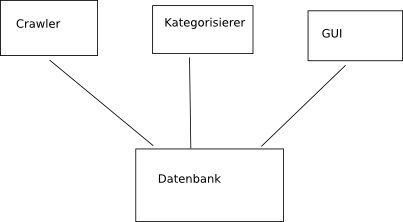
\includegraphics[width=\textwidth]{dia/systemmodell.pdf}
	\caption{Das Systemmodell}
	\label{c:systemmodell}
\end{figure}

\begin{description}
	\item[Crawler] Aufgabe des Crawlers ist es mithilfe der Twitter-Streaming-API Daten von Twitter zu sammeln. Dabei sollen verifizierte Benutzer und Retweets von Tweets dieser Nutzer gefunden werden. Diese Daten sollen noch im Crawler mittels eines Lokalisierungs-Webdienstes lokalisiert werden, bevor sie in der Datenbank abgespeichert werden. Zum detaillierten Entwurf siehe \cref{chap:crawler}.
	\item[Kategorisierer] Um den Crawler so leichtgewichtig wie möglich zu halten, werden die gefunden Accounts von einer weiteren Anwendung, dem Kategorisierer kategorisiert. Unabhängig vom Crawler sucht er in der Datenbank nach Accounts, denen noch keine Kategorie zugeordnet wurde. Anhand der Daten aus der DMOZ-Datenbank sollen diese Accounts dann hierarchisch kategorisiert werden. Dabei können einem Nutzer mehrere Kategorien zugeordnet werden. Der Kategorisierer arbeitet also auf den vom Crawler gefunden Daten und vervollständigt diese. Zum detaillierten Entwurf siehe \cref{chap:kategorisierer}.
	\item[GUI] Die GUI greift lesend und eingeschränkt schreibend auf die Datenbank zu und visualisiert die Daten aus der Datenbank. Dazu gibt der Nutzer Einschränkungen bezüglich von Kategorien und Orten an. Aufgrund dieser Daten werden dann die angeforderten Daten aus der Datenbank geholt und visualisiert. Samit baut die GUI auf Crawler und Kategorisierer auf, welche jedoch unabhängig von der GUI sind. Es ist möglich über die GUI weitere Twitteraccounts (auch nicht verifizierte) in die Datenbank aufzunehmen. Zum detaillierten Entwurf siehe \cref{chap:gui}.
	\item[Datenbank] In der Datenbank werden sämtliche vom Crawler gefundene Daten abgespeichert. Der Kategorisierer vervollständigt diese dann, sodass die Daten in aufbereiteter Form für die GUI zur Abfrage zur Verfügung stehen. Zum detaillierten Entwurf siehe \cref{chap:datenbank}.
\end{description}